\documentclass[12pt]{article}
\usepackage{amsmath, amssymb, amsthm}
\usepackage{latexsym, epsfig, ulem, cancel, multicol, hyperref}
\usepackage{graphicx, tikz, subfigure,pgfplots}
\usepackage{blindtext}
\usepackage[a4paper, total={6in, 8in}]{geometry}
\setlength{\parindent}{0pt}
\usepackage{multirow}
\usepackage{mathtools}
\pgfplotsset{width=10cm,compat=1.9}
\usepackage{amsmath, amssymb, amsthm, graphicx, hyperref}
\usepackage{enumerate}
\usepackage{fancyhdr}
\usepackage{multirow, multicol}
\usepackage{tikz}
\usepackage{comment}

\setlength{\parskip}{1ex}

\newcommand{\T}[0]{\top}
\newcommand{\F}[0]{\bot}
\newcommand{\liminfty}[1]{\lim_{#1 \to \infty}}
\newcommand{\limzero}[1]{\lim_{#1 \to 0}}
\newcommand{\limto}[1]{\lim_{#1}}
\newcommand{\Z}{\mathbb{Z}}
\newcommand{\R}{\mathbb{R}}
\newcommand{\C}{\mathbb{C}}
\newcommand{\Q}{\mathbb{Q}}
\newcommand{\odd}[0]{\mathbb{Z} - 2\mathbb{Z}}
\newcommand{\lineint}[1]{\int_{#1}}
\newcommand{\pypx}[2]{\frac{\partial #1}{\partial #2}}
\newcommand{\divg}{\boldsymbol{\nabla} \cdot}
\newcommand{\curl}{\boldsymbol{\nabla}\times}
\newcommand{\dydx}[2]{\frac{\text{d} #1}{\text{d} #2}}
\newcommand{\sqbkt}[1]{\left[ #1 \right]}
\newcommand{\paren}[1]{\left( #1 \right)}
\newcommand{\tribkt}[1]{\left< #1 \right>}
\newcommand{\abso}[1]{\left|#1 \right|}
\newcommand{\zero}{\{0\}}
\newcommand{\then}{\rightarrow}
\newcommand{\nonneg}{\Z^+ \cup \{0\}}
\DeclarePairedDelimiter\ceil{\lceil}{\rceil}
\DeclarePairedDelimiter\floor{\lfloor}{\rfloor}
\newcommand{\union}[2]{\bigcup_{#1}^{#2}}
\newcommand{\inter}[2]{\bigcap_{#1}^{#2}}
\newcommand{\openclose}[1]{\left( #1 \right]}
\newcommand{\closeopen}[1]{\left[ #1 \right)}
\newcommand{\compo}[2]{#1 e^{i #2}}
\newcommand{\laplase}{\bigtriangleup}
\newcommand{\bra}[1]{\left< #1 \right|}
\newcommand{\ket}[1]{\left| #1 \right>}
\newcommand{\braket}[2]{\left< #1 \mid #2 \right>}
\newcommand{\ketbra}[2]{\left| #1 \right> \left< #2 \right|}
\newcommand{\ketpsit}{\ket{\psi(t)}}
\newcommand{\ketphit}{\ket{\phi(t)}}
\newcommand{\ham}{\mathbf{H}}
\newcommand{\unx}{\hat{\mathbf{x}}}
\newcommand{\uny}{\hat{\mathbf{y}}}
\newcommand{\unz}{\hat{\mathbf{z}}}
\newcommand{\uns}{\hat{\mathbf{s}}}
\newcommand{\unr}{\hat{\mathbf{r}}}
\newcommand{\untheta}{\hat{\boldsymbol\theta}}
\newcommand{\unphi}{\hat{\boldsymbol\phi}}




\newtheorem*{remark}{Remark}
\title{\textbf{Analytical Mechanics}}
\author{Dennis Li}
\begin{document}
\maketitle
\hrule


\section{Newtonian Mechanics}
To start the class off, we will re-formulate our understanding of the Newtonian mechanics, starting from revisiting the Newtons law of motion. 

\subsection{Newton's Laws of Motion}
The first of which is the \textbf{law of inertia}. It helps us define a framework in which motions can be studied in Newtonian settings. We can see it as: 

\textit{A \textbf{reference frame} is \textbf{inertial} if a particle initially at rest stays at rest when no external force is applied}. 


This helps us define where we can apply the second law.

The second law states that if you are in an inertial reference frame and you are measuring physical parameters, the following relationship is true.
\[
\sum \mathbf{F}_{c} = \dydx{\mathbf{p}_{c}}{t}
\]
Here $c$ stands for \textbf{center of mass}. And it is important that we are studying the right hand side of the equation since it leads us to the third law, which can be summarized as: For each action, there is an equal but opposite and co-linear reaction. Written as
\[
\mathbf{F}_{BA} = - \mathbf{F}_{BA}
\]
This law implies that force is dependent of the reference frame, and this is why we have to make some specification in the second law. The \textbf{weak} version does not require it to be \textit{co-linear}.


\subsection{Representation}
Work in Progress

\subsection{Convert Cartesian to Polar in 2D}
Representation in Cartesian coordinates
\[
\unx(x,y)=\unx(0,0)=\unx
\]
And the same applies to $\uny$ since Cartesian coordinates are uniform. And we can represent the position with
\[
\dydx{}{t}\mathbf{r}(t) = \Dot{x}\unx+\Dot{y}\uny
\]
Now we examine what happen if we go to polar form. In polar form, the position vector is expressed simply as
\[
\mathbf{r}(t) = s\uns
\]
Here, we use $s$ to define the distance from the origin in the $2D$ plane. We have to acknowledge that $\uns$ changes depending on where the position vector is, therefore it is not uniform. We have to treat it also as a function of time. The velocity is defined the same way as before, by taking the derivative with respect to time. We obtain 
\[
\Dot{\mathbf{r}} = \Dot{s}\uns + s\Dot{\uns} 
\]
Here, we have to find a way to express this in terms of $\uns$ and $\unphi$. First, we would define our unit polar vectors.
\[
\uns = \cos\phi\unx + \sin\phi\uny
\]
Here, $\phi$ is a function of time. And since $\unr \perp \unphi$, we can use the fact that $\unr \cdot \unphi = 0$ to find $\unphi$. It will be
\[
\unphi = -\sin\phi\unx + \cos\phi\uny
\]
Now, if we take their time derivative, we have
\[
\Dot{\uns} = -\Dot{\phi}\sin\phi\unx + \Dot{\phi}\cos\phi\uny = \Dot{\phi}\unphi
\]
\[
\Dot{\unphi} = -\Dot{\phi}\cos\phi\unx - \Dot{\phi}\sin\phi\uny = - \Dot{\phi}\uns
\]
The result is obtained from doing some substitution. And if we substitute our result into the original expression for $\Dot{\mathbf{r}}$, we have
\[
\Dot{\mathbf{r}} = \Dot{s}\uns + s\Dot{\phi}\unphi
\]
This completes our description to the velocity in polar form. And if we take the time derivative again, we will have the expression for acceleration. Here's how
\begin{align*}
    \dydx{}{t}\Dot{\mathbf{r}} &= \dydx{}{t}\paren{\Dot{s}\uns + s\Dot{\phi}\unphi} \\
    \ddot{\mathbf{r}} &= \ddot{s}\uns + \dot{s}\dot{\uns} + \dot{s}\Dot{\phi}\unphi + s\ddot{\phi}\unphi + s\Dot{\phi}\dot{\unphi}\\
                      &= \ddot{s}\uns + \dot{s}\dot{\phi}\unphi + \dot{s}\dot{\phi}\unphi + s\ddot{\phi}\unphi -  s\Dot{\phi}^2\uns\\
                      &= \paren{\ddot{s}-s\dot{\phi}^2}\uns + \paren{2\dot{s}\dot{\phi}+s\ddot{\phi}}\unphi
\end{align*}



\subsection{Convert Cartesian to Spherical in 3D}

\subsection{Convert Cartesian to Cylindrical in 3D}

\subsection{Dot Products and Cross Products}
There are several things we need to know about these products. First, if we have two vector $\mathbf{a}$ and $\mathbf{b}$. Think of it like follows
\[
\mathbf{a}\cdot\mathbf{b} = \abso{\mathbf{b}}\paren{\mathbf{a}\cdot \Hat{\mathbf{b}}}
\]
Think of it like projecting one vector onto another and re-scaling it using the magnitude. Here, $\hat{\mathbf{b}}$ is the \textit{unit vector} of $\mathbf{b}$, or the normalized $\mathbf{b}$. This way you have a more intuitive understanding of it.

As for the cross product, it creates a third vector that is perpendicular to the plane created by the original 2 vectors. Let us write it out as follows
\[
\mathbf{a}\times \mathbf{b} = \mathbf{c} \quad \mathbf{a}\perp \mathbf{c} \vee \mathbf{b}\perp\mathbf{c}
\]

\section{Changing Between Frame}
If we start with $\mathbf{r},\mathbf{v},\mathbf{a}$, and we moved to another frame and defined as $\mathbf{r}',\mathbf{v}',\mathbf{a}'$. If we have 2 frame of reference $A,B$ with origin at $A,B$, and a mutual object $C$ somewhere else, we can find the following relationship.
\[
\mathbf{r}_{A,B} + \mathbf{r}_{B,C} = \mathbf{r}_{A,C}
\]
And
\[
\mathbf{r}_{C,A} = \mathbf{r}_{C,B} - \mathbf{r}_{A,B}
\]
We should get into the hoppy of using a double subscript to track which frame are we talking about and what frame are we in. For example
\[
\mathbf{r}_{A,B} \colon \text{A relative to B}
\]
Remember that $\mathbf{A} - \mathbf{B}$ essentially gives you a vector pointing from the tip of $B$ to the tip of $A$ when they are connected tail to tail.
What happens is that you can in fact figure out what $C$ is like in another frame, say, $B$, by subtracting the position vector between $B$ to $A$. We can take derivative of the expression to receive
\begin{align*}
    \mathbf{v}_{A,B}+\mathbf{v}_{B,C}=\mathbf{v}_{A,C}\\
    \mathbf{v}_{C,A} = \mathbf{v}_{C,B} - \mathbf{v}_{A,B}
\end{align*}
We do it again to get the acceleration
\begin{align*}
    \mathbf{a}_{A,B}+\mathbf{a}_{B,C}=\mathbf{a}_{A,C}\\
    \mathbf{a}_{C,A} = \mathbf{a}_{C,B} - \mathbf{a}_{A,B}
\end{align*}
This is always true if things are not spinning.

Also notice that if you are trying to find $C,A$, you are essentially subtracting your information of $C$ in $B$ and $A$ in $B$. This is an easier way to memorize it. 

\subsection{Question}
If 2 frames agree with the velocity at one moment, do they have to agree with the acceleration as well?

Think about the \textit{Shoot the Monkey} problem. If you aim a gun at a monkey that will drop off from a tree the moment you shoot at it, you are actually aim directly at the monkey. Since in the monkey's perspective, the bullet is falling along with the bullet once it leaves the muzzle. 

In the Hunter's perspective, the bullet will have the same acceleration downward and falling with the monkey. But in the monkey perspective, there is no acceleration since it is a free-fall frame. The monkey will only see the bullet approaching at constant velocity. 

Therefore, the answer to this question is \textbf{NO}.

\subsection{Equivalence Principle}
If you are in a frame that has acceleration \textbf{a} relative to a inertial frame $S$. Note that all inertial frame agree with acceleration since none of them accelerates with respect to each other, else it would not be inertial. In this case, Newton's Second Law can work if you inject \textit{extra fake gravity} into $S$.

We can use the acceleration of $S$ with respect to the inertial frame $S_i$, we define it as $\mathbf{a}_{S,S_i}$. And we use this acceleration to define a fake force or a \textit{fake gravity}, 
\[
-\mathbf{a}_{S,S_i} = \mathbf{g}_{fake}
\]
and Newton's Second Law works again. 

\section{Moving on a Curve}
The acceleration on a particle moving on a curve can be characterized by
\[
\mathbf{a} = \dydx{\abso{\mathbf{v}}}{t}\hat{\parallel} + \frac{v^2}{r_{osc}}\hat{\perp}
\]
where $v$ is the speed, and $\mathbf{v}$ is the velocity vector. And $r_{osc}$ is the radius of the osculating circle.


\subsection{Expressing Speed}
We can express speed as a function of position, and find the acceleration this way. Think of the function of force be written as following. 
    \[
    F(x_i, \dot{x}_i) = f(x_i) g(\dot{x}_i)
    \]
            Rewrite as
            \[
            m\dydx{^2x_i}{t^2} = f(x_i) g(\dot{x}_i)
            \]
            Then, write it as
            \[
            m\dydx{}{t}\dot{x}_i = f(x_i) g(\dot{x}_i)
            \]
            Now we use the chain rule to rewrite the differential operator
            \[
            m\dydx{}{t}\dot{x}_i  = m\paren{\dydx{}{x_i}\dydx{x_i}{t} }\dot{x}_i= f(x_i) g(\dot{x}_i)
            \]
            And this becomes
            \[
            m\dot{x}_i\dydx{\dot{x}_i}{x_i} = f(x_i) g(\dot{x}_i)
            \]
            Now this is separable, and it yields
            \[
            m\dot{x}_i\frac{d\dot{x}_i}{g(\dot{x}_i)} = f(x_i)\,dx_i
            \]
            And we can integrate this on both side. 

    This means that we can define an equivalence relationship
    \[
    a = v\dydx{v}{x}
    \]
    This is what happens when you have speed as a function of position, and cannot explicitly express velocity as a function of time, such as in a spring motion, where
    \[
    \frac{1}{2}mv^2 - \frac{1}{2}kx^2 = 0
    \]
    Yes, you can obtain the expression of velocity, but that is after solving the ODE. This is not always feasible, so we can use the above property to express acceleration directly using the speed as a function of position. 

\subsection{Exponential Function}
    In physics, a function such as $y = e^{x}$ is not nicely defined since raising e to $5$ meters power is not. Therefore we need to add some coefficient to make the dimensions right, for example.
    \[
    y(t) = Ce^{kt}
    \]
    Where $C$ has unit of $L$ length, and $k$ has unit of $\frac{1}{L}$ length.
    \subsubsection{Example 1}
    If a particle traces this path, and remains at a constant speed $v_0$, how do we figure out its acceleration? Since we have no information on their relationship with respect to time, we can differentiate it implicitly
    \[
    \dot{y} = \dydx{y}{t} = \dydx{y}{x}\dydx{x}{t} = Cke^{kx}\dot{x}
    \]
    We can this again, and differentiate
    \[
    \ddot{y} = \dydx{\dot{y}}{t} = \dydx{\dot{y}}{x}\dydx{x}{t} = Ck^2e^{kx}\dot{x} + Cke^{kx}\ddot{x} = Cke^{kx}\paren{k\dot{x}^2+\ddot{x}}
    \]
    We also know that $\mathbf{a}\perp\mathbf{v}$. Therefore we can use the fact 
    \[
    \dot{x}\ddot{x}+\dot{y}\ddot{y} = 0
    \]
    This is the last piece of the puzzle for us to figure out the acceleration. 
    \subsubsection{Example 2}
    If the particle is released from $kx=1$ and this trajectory is frictionless where the particle has to move along it, what is its acceleration and velocity at $x=0$? In this case, we can exploit the fact that
    \[
    K(t) + V(t) = \textit{Constant}
    \]
    We can in fact implicitly differentiate this constraint to obtain
    \[
    \dydx{}{t}\paren{ \frac{1}{2}v^2(t) + gy(t)} = 0
    \]
    Consequently, this gives us
    \[
    v\dot{v} + gv_y = 0
    \]
    This eventually gives you
    \[
    \dydx{v}{t} = \frac{-g v_y}{v}
    \]
    And we can work from here.




\section{Newton's Second Law}
    When we are really using this law, we are actually working with a vector ODE
    \[
    \mathbf{F}_{net} = m\ddot{\mathbf{r}}
    \]
    There are a few scenarios where we can work on it. First of which it becomes an algebraic equation with some elementary problems.

    Another scenario is where we would obtain some ODE from it, such as in harmonic oscillators. 
        \[
        -k\mathbf{x} = m\ddot{\mathbf{x}}
        \]

    A third scenario, we would have drag and air resistance, something like
    \[
    \mathbf{F} = \mathbf{F}(\mathbf{v})
    \]
    This becomes a first order ODE with components of $\mathbf{v}(t)$ to obtain $\mathbf{r}(t)$.

    We would never go beyond second order. But we might have a mix of them where we have a system of ODE. This is what the Newton's Second Law is the most powerful. 

    For example, for a particle moving a electromagnetic field, how would we express its motion?

\ubsection{Motion in B Field}
    For details, check chapter $2$ of Taylor. Say you have a particle in a uniform \textbf{B} field in the $\unz$ direction. 
    \[
    \mathbf{B} = B_0 = \unz
    \]

    You have a particle with velocity 
    \[
    \mathbf{v}_0  = v_{x0}\unx +v_{y0}\uny + v_{z0}\unz 
\] 
at time $t=0$. We want to find $x(t),y(t),z(t)$. We know that the force can be written as
\[
\mathbf{F} = m\ddot{\mathbf{r}} = q\mathbf{v}\times \mathbf{B}
\]
do cross products as cyclic permutations and not the determinant, its faster. And we have obtained that the force the particle experiences in the field is
\[
\begin{cases}
    m\ddot{x} = qv_yB_0\\
    m\ddot{y} = qv_xB_0\\
    m\ddot{z} = 0
\end{cases}
\]
We have obtained the ODE
\[
\dot{v}_x = \frac{qB_0}{m}v_y \quad \dot{v}_y = -\frac{qB_0}{m} v_x
\]
We will give the coefficient a name $\omega = \frac{qB_0}{m}$, since it should have a unit of $s^{-1}$. We will solve this with a tricky method. We differentiate the first equation and obtain
\[
\ddot{v}_x = \omega\dot{v}_y = -\omega^2v_x
\]
And we know what $\dot{v}_y$ is, we can simplify it. Do the same for the other ODE
\[
\ddot{v}_y = -\omega v_x = -\omega^2v_y
\]
This is obviously a harmonic oscillator equation and its solution is well-known. 
\[
\begin{cases}
    v_x = A\sin\omega t + B\sin\omega t\\
    v_y = C\sin\omega t + D\sin\omega t
\end{cases}
\]
Now we throw our initial condition in, that is the speed at $t=0$. Since it was second order, we will differentiate the solution and throw in $t=0$ and compare it with out acceleration. Then we will figure out what the coefficients are. 

\subsection{Drag}
Now we would like to include drag in our system to make it extra fun. Say we have a drag
\[
\mathbf{F}_d = -b\mathbf{v}
\]
Where $b$ has the dimension $kg/s$. 

Here, think of this scenario. A mass moving in $\unx$ with some speed $v_0$. And we have a linear drag, the air resistance $-\unx$. Intuitively, the block will keep slowing down at a rate proportional to its speed. And when it stops, there are no more drag and this will take indefinite amount of time. We can write down the following info
\[
\mathbf{F}_{net} = m\dot{\mathbf{v}} = -b\mathbf{v}
\]
Therefore
\[
\dot{\mathbf{v}} = -\frac{b}{m}\mathbf{v} = -\frac{1}{\tau}\mathbf{v}
\]
Where $\frac{1}{\tau} = \frac{b}{m}$, because it has the dimension $s^{-1}$. And now we pick a frame, where we already sort of defined previously. 

Be very mindful that when we start to write ODEs, we are only working with scalar. Here we can start writing down euqatoins
\[
\dot{v}_x = -\frac{1}{\tau}v_x
\]
This is obviously $v_x = Ce^{-\frac{t}{\tau}}$, where $C$ is $v_0$. This can be extrapolated from the initial condition. Now, to obtain the position, simply integrate it
\[
x = -v_0\tau e^{-\frac{t}{\tau}} + C
\]
If we throw in $t=0$, we know $x=0$. And this tells us that $C = v_0\tau$. How do we interpret this result?
\[
x(t) = v_0\tau\paren{1 - e^{-\frac{t}{\tau}}}
\]
Basically this represents how far this object would have gone in time $\tau$ if not the resistance of air. 

The reason why we know $\frac{1}{\tau}$ goes into the coefficient is because the exponents need to be dimensionless. This coefficient has to cancel the unit of time on the exponent. This is why we have $\frac{t}{\tau}$

And if we think about what the trajectory of one dimensional motion with drag is like, we can figure out that it is
\[
\mathbf{v}(t) = \mathbf{v}_0 e^{-\frac{t}{\tau}} + \mathbf{v}_{ter}\paren{1-e^{-\frac{t}{\tau}}}
\]

Think of it as the initial velocity would die out exponentially and the velocity will slowly be stabilized at $\mathbf{v}_{ter}$. If we want something to have big impact at start but die-out quickly, we just slap an exponential function in front of it. Try to throw in different value for initial velocity and think about the behavior of the velocity. 
If the initial velocity is $0$, we have the free falling with drag expression.
If the initial velocity is opposite to the direction of the gravity, the gravity and the drag will point into the same direction and die out quickly and exponentially, the velocity will still approach terminal velocity. So think of it like an exponential function that starts below the $t$ axis at $t=0$. It will cross $v=0$ quickly, and \textit{accelerate} to terminal velocity.

And if were to integrate this and try to find the constant of integration, we have
\[
\mathbf{y}(t) = \mathbf{v}_{ter}t + \paren{1-e^{-\frac{t}{\tau}}\paren{\mathbf{v}_{0}-\mathbf{v}_{ter}}}\tau + \mathbf{y}_0
\]
Since we did everything with a vector, now we can just integrate that extra fake gravity and realize that
\[
\mathbf{v}_{ter} = \mathbf{g}_{ef}\tau
\]
Figure out the combined, or effective gravity. Now we can use the same \textit{drag} formula. 

\subsection{More Drag}
Now we add friction. We recognize that the frictional force, defined by
\[
F_k = \mu_k = mg\mu_k
\]
We see that this is exactly like tossing stuff straight up. So this is just what we have done before.
\[
\mathbf{v}(t) = \mathbf{v}_0e^{-\frac{t}{\tau}} + \mu_k\tau\paren{1-e^{-\frac{t}{\tau}}}
\]

\textbf{Important Note:} An important takeaway is to think of a problem and compare it to something we have learned instead of solving everything from scratch. 

\subsection{Tossing With Drag}
Now we toss a ball in the air with angle $\theta$. WIth gravity as well. The $\unx$ component is the same as before, and the $\uny$ component is the toss up and down situation. We can obtain the system as
\[
m\dot{\mathbf{v}} = m\mathbf{g} - b\mathbf{v}
\]
If we break it up into components, we have
\[
\begin{cases}
    x\colon = -\frac{1}{\tau}v_x = \dot{v}_x\\
    y\colon -g-\frac{1}{\tau}v_y = \dot{v}_y
\end{cases}
\]
And if the drag is not linear, say
\[
\mathbf{F}_d = -c\abso{\mathbf{v}}\mathbf{v}
\]
Read \textit{Taylor} and \textit{Marion \& Thornton}. We can still extract some information out of a non-linear coupled ODE. If one would like to investigate and do a project on it, it would be a fun one. 

\section{Energy}
We need to revisit the idea of \textbf{Potential Energy}. We need to know that the potential energy is associated with the \textbf{Configuration} of the system.

For example, $U_g = mgh$ is an oversimplification that we use, because the energy is from the way a particle is located with respect to the earth. It is not an intrinsic property of a certain particle, but a system.

\subsection{Work-Energy Theorem}
\subsubsection{Conservative Force}
We need to know what sort of force we call is conservative forces
\begin{enumerate}
    \item It is a force that depends on where the particle is
    \[
    \mathbf{F} = \mathbf{F}(\mathbf{r})
    \]
    
    \item Work done on a particle as you go from $A$ to $B$ is independent of the path it takes. 
    \[
    W = \int_C \mathbf{F}\cdot \text{d}\mathbf{r}
    \]
    Here, as long as $C$ goes from $A$ to $B$, the work is constant. 
    
    \item The curl of a conservative vector field is $0$.
    \[
    \curl \mathbf{F} = 0
    \]
    And we can also write the vector field as the gradient of some scalar function
    \[
    \mathbf{F}(\mathbf{r}) = -\boldsymbol{\nabla}U(\mathbf{r})
    \]
\end{enumerate}

\subsection{One Dimensional Motion}
Ideally, we want to treat things as one dimensional motion. Because if we only consider one dimensional motion
\[
\curl \mathbf{F} = 0
\]
This is always true because there is no $y$ and $z$ direction of motion. In this case, 
\[
F(x) = -\dydx{U}{x}
\]
\subsection{First Technique}
The main take-away, or technique is that How to read a potential energy diagram.

Imagine we have some random function that is our potential $U(x)$, the places where a particle experiences no force is the local max and min. This understanding carries over to an actual photograph of mountains and hills. The apex and valley is the only place where a particle can stay still. Also the saddle points. You can understand this by knowing that the derivative on the local max and min is $0$. 

\begin{figure}[!h]
    \centering
    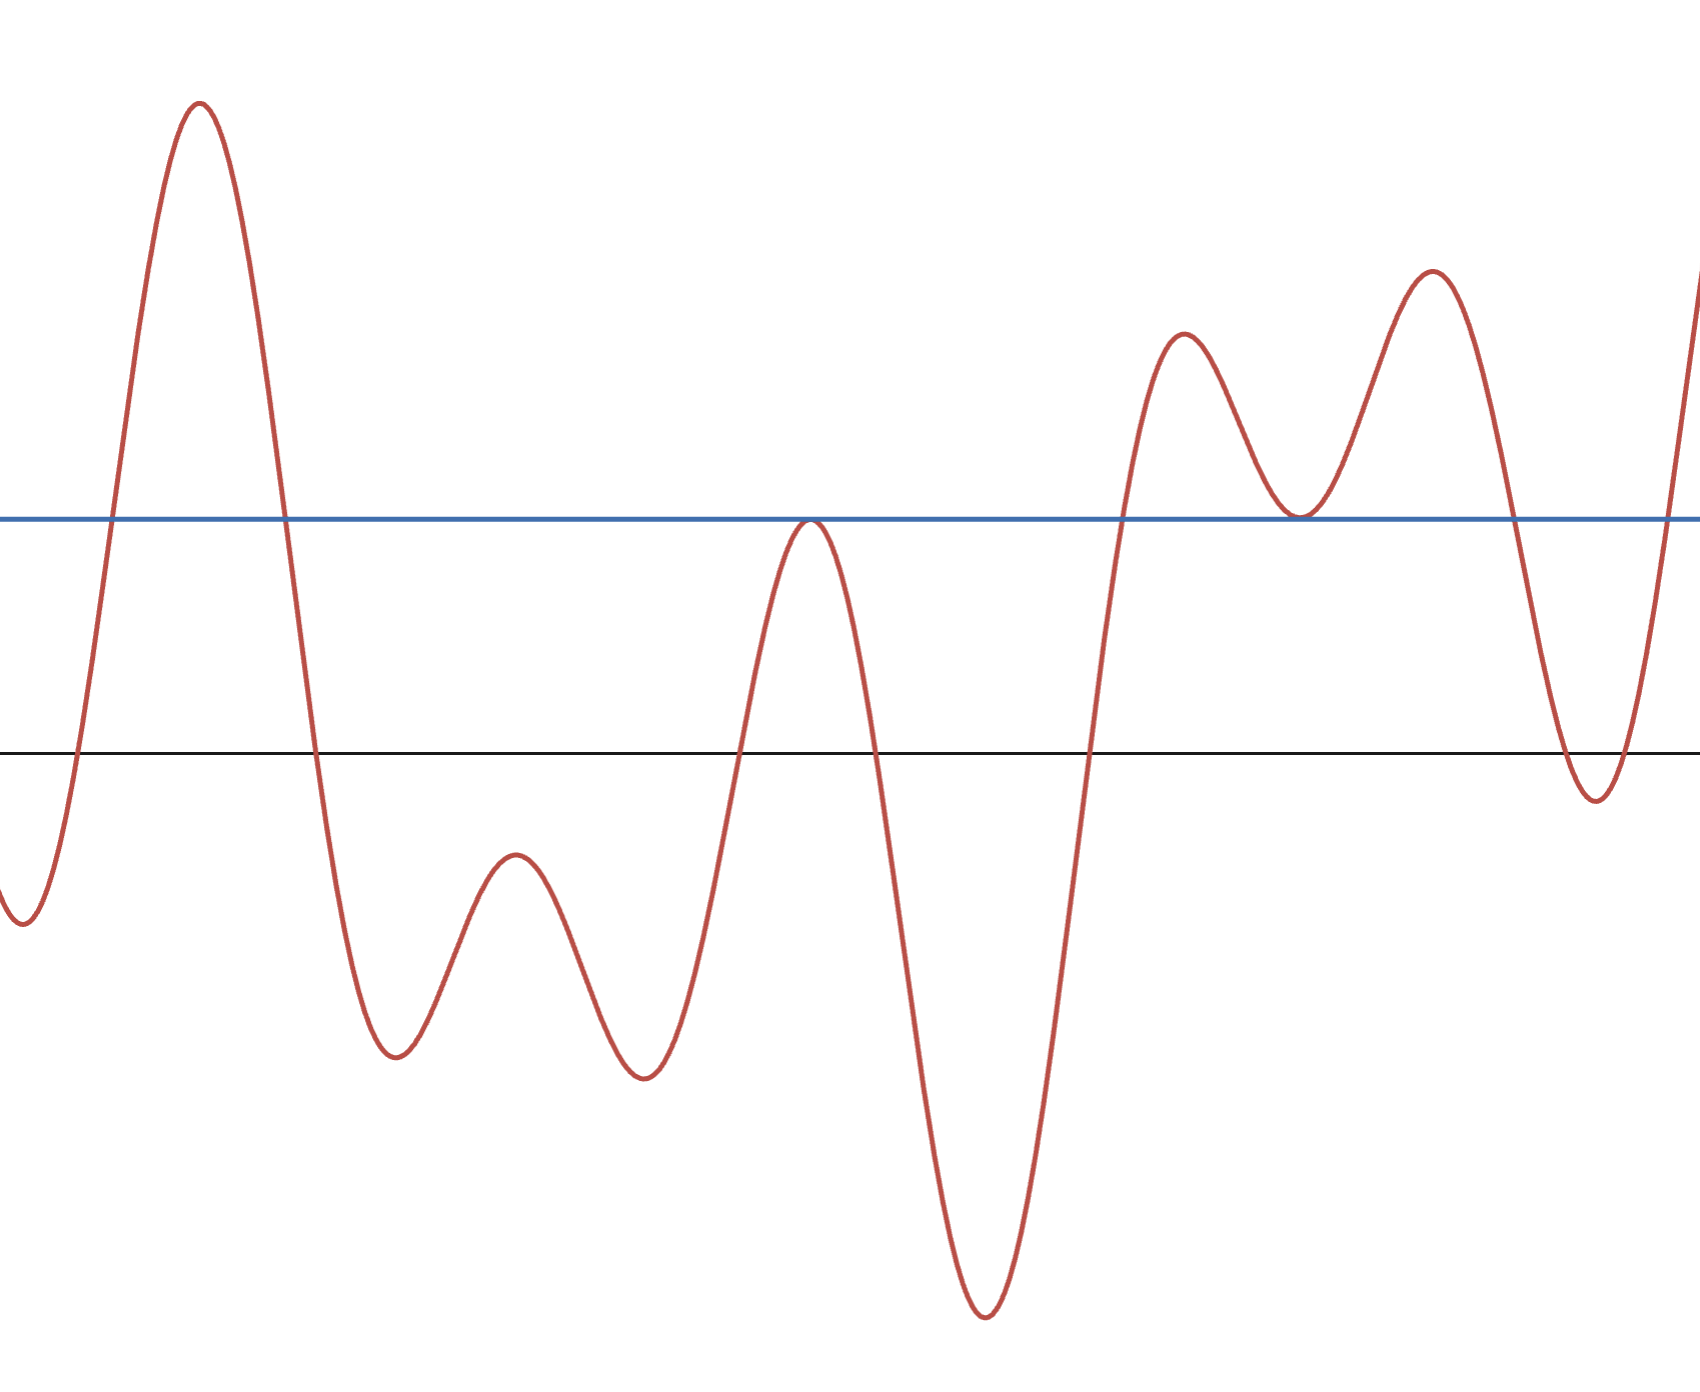
\includegraphics[width=0.5\linewidth]{Pictures//NotesPic/PotentialPic.png}
    \caption{A potential graph}
    \label{fig:potential_pic}
\end{figure}

You can draw a horizontal line, and this will give you the region which the particle would have access to, cuz your potential cannot go more than what you had.

And if you would travel from one peak to another peak that is on the same height, it would actually take you \textit{infinite} amount of time. You will approach it asymptotically, but will take an indefinite amount of time to get there. 

And if you are in a valley, your motion will be like a Harmonic Oscillator. 

So if we treat stuff like one dimensional object, and plot the potential graph, small disturbances in the potential is best modeled as the harmonic oscillator. 

The way we do it is use the best fit parabola found by Taylor Series expansion. Let $u(x)$ be our function of potential with respect to position, and $x_0$ be the place of interest.
\[
u(x) = u(x_0) + u'(x)(x-x_0) + \frac{1}{2}u''(x)(x-x_0)^2 + \ldots
\]
If we are in a valley, the first derivative is effectively gone, leaving us with the second order term, and we ignore all higher orders. Now we have a parabolic approximation that models a harmonic oscillator.

So how do we find the period of such motion? we can do that with the following procedure.
\[
E_{tot} = \frac{1}{2}mv^2(x) + u(x)
\]
Now we want to rewrite everything
\[
\frac{2}{m}\sqbkt{E_t - u(x)} = v^2(x) = \paren{\dydx{x}{t}}^2
\]
We can obtain the following
\[
dt = \sqrt{\frac{m}{2}}\frac{dx}{\sqrt{E_t - u(x)}}
\]
Now we can integrate
\[
\int_0^{\frac{T}{2}} \,\text{d}t = \int_{x_{min}}^{x_{max}}  \sqrt{\frac{m}{2}}\frac{\text{d}x}{\sqrt{E_t - u(x)}}
\]
This is effectively
\[
T = \sqrt{2m}\int_{x_{min}}^{x_{max}} \frac{\text{d}x}{\sqrt{E_t - u(x)}}
\]
We can see that if we are trying to integrate from one hill to another hill with the same energy, the integral diverges and this implies that it takes an indefinite amount of time to reach the other endpoint. 

\subsection{Questions That Can Be 1D}
We can actually use this trick to work with a pendulum, Since its path is fixed on a curve, and it is technically a one dimensional path. We need to track where it is on the curve, we use
\[
l\theta = s
\]
Where $l$ is the length of the pendulum, and $s$ is the arc length. We set the lowest point of the pendulum to be the point where potential is $0$. We know that
\[
U(\theta) = mgh = mgl(1-\cos\theta)
\]
We also know that the kinetic energy is
\[
K(\theta) = \frac{1}{2}mv^2 = \frac{1}{2}ml^2\dot{\theta}^2
\]
We obtained this by the below relationship
\[
v = \dydx{s}{t} = l\dydx{\theta}{t}
\]
If we are to graph the function of the potential onto a graph, we have
\begin{figure}[!h]
    \centering
    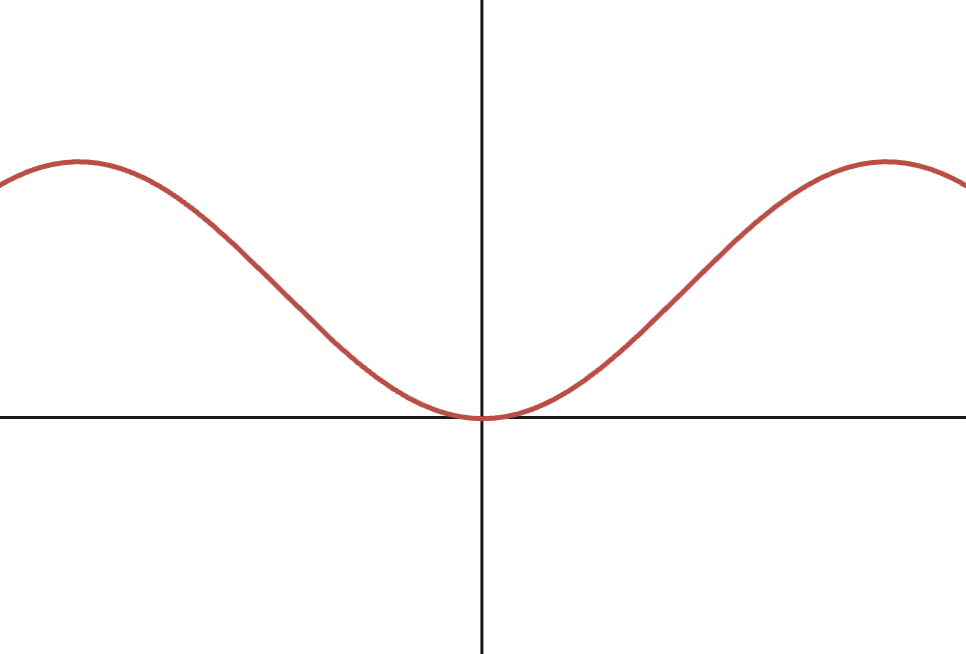
\includegraphics[width=0.5\linewidth]{Pictures//NotesPic/pendulumPotential.png}
    \caption{Potential of a pendulum}
    \label{fig:pendulumpotential}
\end{figure}
WE can see that as long as we have periodic motion for a very big region confined in $-\pi$ to $\pi$.

As long as we can write a system as something that looks like
\[
\begin{cases}
    K = \frac{1}{2}\paren{m_{eff}}\dot{\mathbf{r}}^2\\
    U \approx U_{eq} = \frac{1}{2}\paren{\quad}\dot{\mathbf{r}}^2
\end{cases}
\]
We also define $U'' = k_{eff}$, the effective kinetic energy is the second derivative of the potential. And whatever is in the kinetic energy between the one half and the velocity, it is our effective mass. We can find the angular frequency
\[
\omega^2 = \frac{K_{eff}}{m_{eff}}
\]

We can exploit this relationship. Now lets do some practices. 

Think of a cube on a cylinder rocking back and forth, we can write its height as
\[
y = (r+b)\cos\theta + r\theta\sin\theta
\]
And horizontal movement as
\[
x = (r+b)\sin\theta-r\theta\cos\theta
\]
Now we can obtain the expression for potential energy
\[
u(\theta) = mgy = mg\sqbkt{(r+b)\cos\theta + r\theta\sin\theta}
\]
and now we can take derivativees of the poential energy to learn about it
\[
u' = mg\sqbkt{-b\sin\theta + r\theta\cos\theta}
\]
We see that the thing has equilibrium at
\[
\tan\theta = \frac{r}{b}\theta
\]
This means that when the radius $r$ is bigger than the length of the block $b$, we can obtain 3 points where the block can stay stationary.

We can examine the second derivative
\[
u'' = mg\sqbkt{-b\cos\theta - r\theta\sin\theta+r\sin\theta}
\]
We can see the equilibrium is
\[
u''(0) = mg\paren{r-b}
\]
We can see that the equilibrium is stable if $r>b$, not stable if $b>r$. Now we have plenty of information about the block. 

We see how much we have learned by simply looking at the equation of the potential energy of a cube on a cylinder. 

And now how do we know its kinetic energy, what is its equation. 

We have to know what is kinetic energy of the system and how do we define it. The claim is, it can be written as
\[
K_t = K_c + K_a
\]
Where $K_t$ is the total kinetic energy of the system. $K_c$ is the kinetic energy of the center of mass. $K_a$ is the kinetic energy of everyone in the frame of the center of mass. 

This is basically what we do in Lagrangian mechanics. We want to express energy with as little coordinates as possible, try to make your calculation and life easier. 

In general, you will always get something that looks like
\[
K = \frac{1}{2}\paren{m_{eff}}\dot{\theta}^2 + \paren{\quad} \dot{\theta}^2
\]
\[
P = \frac{1}{2}\paren{k_{eff}}\theta^2
\]
And the angular frequency is
\[
\omega^2 = \frac{k_{eff}}{m_{eff}}
\]
\subsection{System}
We first need to know how to analyze the center of mass. We define it to be 
\[
M_{tot}\mathbf{r}_{com} = \sum m_i\mathbf{r}_i
\]
We define it this way such that if we differentiate it with respect to time, we have
\[
\dydx{}{t}\paren{M_{com}\mathbf{r}_{tot} = \sum m_i\mathbf{r}_i}
\]
This gives us
\[
M_{tot}\mathbf{v}_{com} = \sum m_i \mathbf{v}_i
\]
Do this process again, we would obtain
\[
M_{tot}\mathbf{a}_{com} = \sum m_i \mathbf{a}_i
\]
If we examine the term $m_i\mathbf{a}_i$, we find that this is the net force on the $i$-th particle. We know that this net force is as follows
\[
\mathbf{F_i} = \mathbf{F}_{net,i} + \mathbf{F}_{i,j}
\]
Where $j$ is some other particle in the same system. This means that if we sum it up and obtain something for the entire system, we realize that all these internal forces cancels. Therefore we only care about the external forces. 

Recall the the \textbf{Work Energy Principle} suggests that
\[
\sum W = \Delta E
\]
We only care about the changes in total energy of all particles, and we call that work. 

Therefore 2 different approaches. 
\begin{enumerate}
    \item We can only consider work done on the center of mass, and understands that it is equivalent to the change of energy of the center of mass, which is the change of potential and kinetic energy of the center of mass. This is the single particle version of the center of mass.
    \item The alternative is legitimately doing the work on individual particles to figure out the total changes. This means that we want to track the change of energy externally and internally, and it should be equivalent to the work done on individual particle. 
    \[
    W_{i} = W_{ext,i} + \sum_{j\neq i} W_{i,j}
    \]
    In this case, we have to consider the internal energy. Now we have to consider this exact situation for every single particle
    \[
    W(\text{work on all particle}) = W(\text{external force on all particle}) + W(\text{all internal work})
    \]
    Every time a system changes its configuration or shape, the second term is usually non-zero. This is why we want to introduce the term \textbf{rigid body}. 

    A \textbf{rigid body} is where the internal particles are not moving with respect to each other. There are no internal work.

    Usually, when we see this term, we accept that the net internal work will be zero. 
\end{enumerate}

A very important thing to know is that you have to use the work energy theorem to show that the energy is conserved before we can use these fact such as energy conservation. We cannot just assume it is true on any system, its something we need to show explicitly. 






















\end{document}